\section{Theorie}

Die Tomographie ist ein bildgebendes Verfahren, das ein Objekt schichtweise darstellt. Strahlung, hier Gammastrahlung, durchdringt das Objekt und liefert durch die bekannte Eingangsintensität $I_0$, die gemessenen Intensitäten $N_j$ und die gemessenen Wegstrecken $d_{j,i}$ die daraus resultierenden Absorptionskoeffizienten $\mu_i$, mit denen sich das Material identifizieren lässt. 
Der Zusammenhang der zuvor genannten Größen lautet für $j$ Messungen
\begin{equation*}
    N_j = I_0 \, \exp\left(- \sum_{i} \mu_i \, d_{j,i} \right).
\end{equation*}
Durch Umformung ergibt sich dann die Gleichung 
\begin{equation}\label{eq:linearKoeff}
    \sum_i d_{i,j} \, \mu_i = \ln \left( \frac{I_0}{N_j} \right),
\end{equation}
bzw. in Matrixschreibweise 
\begin{align}\label{eq:LGS_mu}
\mathbf{A} \cdot \symbf{\mu} = \mathbf{I}.
\end{align}
Die Matrix $\mathbf{A}$ enthält dabei die jeweiligen Weglängen, der Vektor $\mathbf{I}$ entspricht den Elementen $\ln\! \left( \frac{I_0}{N_j} \right)$ und der Vektor $\symbf{\mu}$ enthält die Absorptionskoeffizienten.
Hier wurden $i$ kleine Würfel in einem großen Würfel angeordnet. Dabei bezieht sich der Absorptionskoeffizient $\mu_i$ auf den $i$-ten Würfel.
Die Inverse der Matrix $\mathbf{A}$ und der Vektor $\mathbf{I}$ lassen sich nicht aufeinander anwenden. Daher werden beiden Seiten mit $\mathbf{A^T}$ erweitert. Dadurch kann jetzt invertiert werden und es ergibt sich der Ausdruck 
\begin{equation*}
    \symbf{\mu} = \left( \mathbf{A^T} \mathbf{A} \right)^{-1} \mathbf{A^T} \mathbf{I}.
\end{equation*}
Die Varianzen der Absorptionskoeffizienten ergeben sich über die Varianzen der gemessenen Intensität $\sigma_{\mathbf{I}}^2$ und die Matrix $\mathbf{V_{I}}$ hat eben diese auf der Diagonalen stehen.
Die resultierenden Varianzen der Absorptionskoeffizienten stehen dann auf der Diagonalen der Matrix $V[\mu]$, die sich zu 
\begin{equation}\label{eq:kov}
    \mathbf{V}[\symbf{\mu}] = \left(\mathbf{A}^T\mathbf{V}^{-1}[\mathbf{I}]\mathbf{A}\right)^{-1}
\end{equation}
ergibt.

Die Gammastrahlung wechselwirkt mit Materie auf drei Arten. Der dominierende Prozess in diesem Energiebereich ist der Photoeffekt. Der Compton-Effekt wird hier hauptsächlich als Hintergrund gemessen und für die Paarbildung muss die Energie des Photons bei der zweifachen Masse des Elektrons liegen.  
Eine exemplarische Darstellung der Wirkungsquerschnitte dieser drei Prozesse ist in Abb. \ref{abb:wirkungsquerschnitt} dargestellt.

\begin{figure}
    \centering
    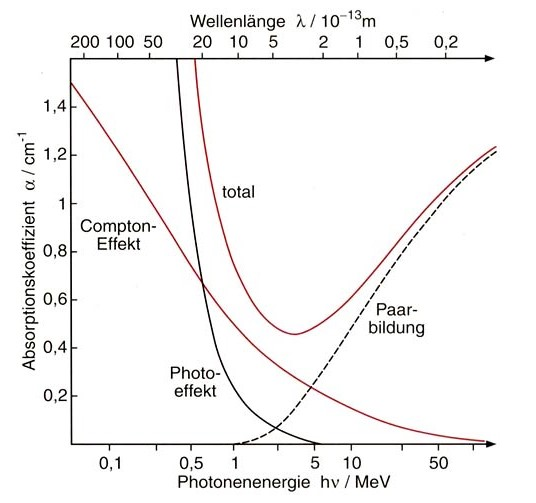
\includegraphics[width=0.6\textwidth]{figures/strahlung.jpg}
    \caption{Beiträge von Photoeffekt, Compton-Effekt und Paarbildung zum Absorptionskoeffizienten von Blei in Abhängigkeit von der Photonenenergie. \cite{strahlung}}
    \label{abb:wirkungsquerschnitt}
    \end{figure}